\documentclass[a4paper,12pt]{article}

\usepackage{geometry}
\usepackage{graphicx}
\usepackage{amsmath}
\usepackage{siunitx}
\usepackage{float}
\usepackage{booktabs}
\usepackage{multirow}
\usepackage{setspace}
\doublespacing

\geometry{margin=1in}

\title{Engineering Part}
\author{Yuze Jiang}
\date{April 2026}

\begin{document}

\maketitle

\section{Powertrain Design}

\subsection{Powertrain Overview}

\subsubsection{Design Objective}

This project focuses on the design of a powertrain system for a Formula Student race car, specifically targeting the \SI{75}{\meter} straight-line acceleration event.

The objective of this event is to minimise the time required to travel a short straight-line distance, under the constraints imposed by the Formula Student UK rules, including a maximum power limit of \SI{80}{\kilo\watt} and a current limit of \SI{500}{\ampere}.

Within these constraints, the powertrain system must efficiently convert electrical energy from a supercapacitor-based storage system into mechanical torque at the wheels, in order to maximise acceleration performance.

\subsubsection{Problem Definition}

Vehicle mass is a primary factor in determining acceleration performance, as increased mass directly reduces the achievable acceleration for a given power level. Minimising system weight while maintaining sufficient power capability and structural robustness is therefore a key design challenge.

The use of a supercapacitor-based energy storage system introduces additional complexity, as the supply voltage decreases during discharge. This affects the available power throughout the acceleration event and requires careful consideration in both powertrain and control system design.

In addition, the system must comply with safety requirements defined by the Formula Student rules. The shutdown circuit (SDC) provides fail-safe protection through independent hardware, operating separately from the controller to ensure safe system shutdown in fault conditions.

Other factors, such as cost and component lead time, must also be considered. Traction-related effects, such as slip, are addressed within the control strategy, and these factors are treated as secondary considerations in this acceleration-focused design.

\subsubsection{Powertrain Structure}

\begin{figure}[H]
    \centering
    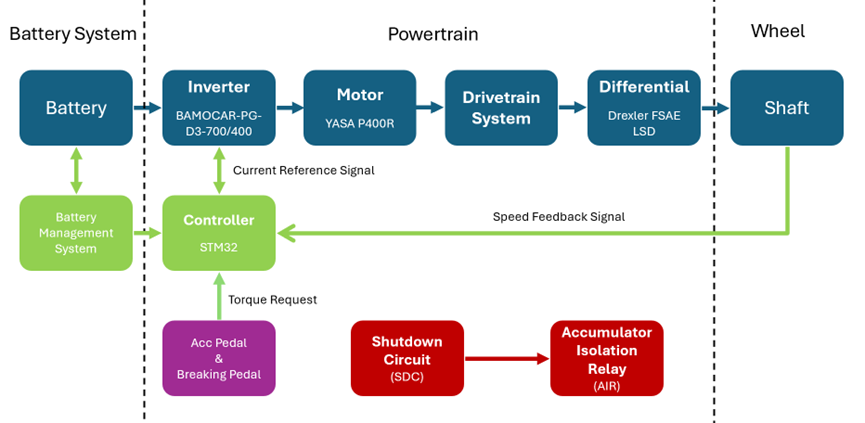
\includegraphics[width=0.8\textwidth]{powertrain_block_diagram.png}
    \caption{Block Diagram for Powertrain System}
    \label{fig:powertrain}
\end{figure}

The powertrain system considered in this work focuses on the components between the accumulator (battery system) and the output shaft, as illustrated in Figure~\ref{fig:powertrain}.

Electrical energy is supplied from the accumulator to the inverter, which converts DC electrical power into controlled AC power for the motor. The motor generates torque, which is transmitted through the drivetrain system and differential to the output shaft, delivering mechanical power to the wheel assembly, which is considered external to this work.

The control system operates in parallel with the powertrain hardware. Driver inputs from the accelerator and brake pedals are processed by the controller, which generates a torque request. This torque request is converted into a current reference signal and sent to the inverter, which regulates motor current to achieve the desired torque output.

Feedback from the powertrain hardware, in the form of shaft or wheel speed, is returned to the controller as a speed feedback signal. This enables the controller to enforce system constraints and maintain stable operation.

In addition to the control system, a shutdown circuit (SDC) provides an independent safety mechanism implemented using non-programmable hardware. When triggered, it actuates the accumulator isolation relay (AIR) to disconnect the tractive system, ensuring fail-safe operation.

Overall, the system is designed to transfer energy efficiently from the accumulator to the output shaft while maintaining controllability and safety.


\subsection{Motor Selection}

\subsubsection{Motor Configuration}

The powertrain architecture adopts a centralised single-motor configuration, as determined by the overall vehicle design.

A multi-motor configuration can provide advantages such as torque vectoring and improved traction control. However, for the \SI{75}{\meter} acceleration event, the vehicle primarily operates under straight-line conditions, where the benefits of torque vectoring are limited.

The selected single-motor configuration reduces drivetrain complexity and vehicle mass, which is beneficial for acceleration performance under power and current constraints. It is therefore used as the basis for subsequent motor selection and powertrain design.

\subsubsection{Motor Requirements}

The motor must be capable of delivering high torque, particularly at low speeds, to maximise usable traction.

It must operate within the \SI{80}{\kilo\watt} power limit and \SI{500}{\ampere} current constraint, requiring a balance between torque output and electrical demand. In addition, compatibility with a variable voltage supply is required due to the use of a supercapacitor-based energy storage system.

Consideration is also given to system mass, cooling requirements, and integration with the inverter and drivetrain, as these factors influence overall performance and packaging.

\subsubsection{Candidate Motors}

Two motor families were considered for the powertrain design: the YASA P400R and the EMRAX 208 series. The EMRAX 208 is available in both medium and high voltage variants, with different cooling configurations including air, liquid, and combined cooling.

\subsubsection{Selection Criteria}

The motor selection is based on a set of weighted criteria reflecting both performance requirements and practical considerations, as summarised in Table~\ref{tab:motor_selection}.

Peak torque is assigned the highest weighting, as it directly determines the ability to generate traction and achieve high acceleration.

Power density is considered as a secondary performance indicator, influencing system mass and packaging.

Voltage compatibility is prioritised due to the variable voltage characteristics of the supercapacitor system.

Cooling requirements, cost, and lead time are assigned lower weightings, as they have limited impact on short-duration acceleration performance.

\subsubsection{Evaluation}

\begin{table}[H]
\centering
\small
\renewcommand{\arraystretch}{1.5}
\setlength{\tabcolsep}{4pt}

\caption{Merit Matrix for Motor Selection}
\label{tab:motor_selection}

\begin{tabular}{lccccccc}
\toprule
\textbf{Criteria} 
& \shortstack{EMRAX \\ MV Air} 
& \shortstack{EMRAX \\ MV Liquid} 
& \shortstack{EMRAX \\ MV Comb} 
& \shortstack{EMRAX \\ HV Air} 
& \shortstack{EMRAX \\ HV Liquid} 
& \shortstack{EMRAX \\ HV Comb} 
& \shortstack{YASA \\ P400R} \\
\midrule
Cost & 2 & 2 & 2 & 1 & 1 & 1 & 0 \\
Lead Time & 1 & 1 & 1 & 1 & 1 & 1 & 0 \\
Power Density & 1 & 1 & 1 & 1 & 1 & 1 & 1 \\
Peak Torque & 0 & 0 & 0 & 0 & 0 & 0 & 3 \\
Voltage Compatibility & 2 & 2 & 2 & 1 & 1 & 1 & 2 \\
Cooling System & 3 & 1 & 2 & 3 & 1 & 2 & 2 \\
\midrule
\textbf{Overall Score} & 21 & 13 & 17 & 18 & 10 & 14 & 22 \\
\bottomrule
\end{tabular}
\end{table}

The results show that the YASA P400R achieves the highest overall score, primarily due to its superior peak torque performance, which has the greatest influence on acceleration capability.

Although the EMRAX 208 variants exhibit higher power density, their lower torque output reduces their effectiveness for this application. Voltage compatibility further supports the selection of the YASA motor under the variable supply conditions.

\subsubsection{Final Decision}

Based on the evaluation, the YASA P400R is selected as the motor for the powertrain system, providing the most suitable solution for the defined performance requirements.

\subsection{Inverter Selection}

\subsubsection{Inverter Requirements}

The inverter must be compatible with the overall powertrain system, ensuring effective operation with the selected motor under the defined electrical constraints.

A key requirement is the ability to operate over a wide input voltage range, allowing flexibility in the design of the supercapacitor-based energy storage system, where the supply voltage varies during discharge.

The inverter must also support the required current and power levels while maintaining reliable integration within the powertrain system.

\begin{figure}
    \centering
    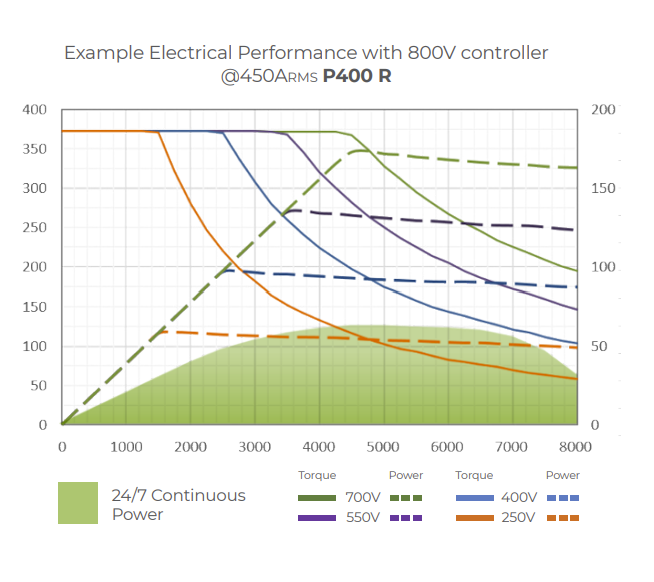
\includegraphics[width=0.5\linewidth]{YASA_Motor_Operation_Graph.png}
    \caption{YASA P400R Operation Curve}
    \label{fig:placeholder}
\end{figure}
\subsubsection{Candidate Inverters}

Several inverter options were considered for the powertrain system, including the DMC544, BAMOCAR PG-D3 series, CM200DX, and CM200DZ.

These candidates provide different voltage ranges, current capabilities, and system integration characteristics, forming the basis for further evaluation. The key specifications are summarised in Table~\ref{tab:inverter_parameters}.

\subsubsection{Candidate Parameters}

\begin{table}[H]
\centering
\caption{Parameters of Candidate Inverters}
\label{tab:inverter_parameters}
\begin{tabular}{lcccccc}
\toprule
Inverter & $V_{\text{max}}$ (V) & $V_{\text{min}}$ (V) & $I_{\text{peak}}$ (A) & $P_{\text{peak}}$ (kW) & Weight (kg) & Cost (USD) \\
\midrule
DMC544 & 450 & 12 & 600 & 300 & 15.3 & 24000 \\
BAMOCAR 400/400 & 400 & 12 & 285 & 75 & 8.5 & -- \\
BAMOCAR 700/250 & 700 & 12 & 178 & 85 & 8.5 & -- \\
BAMOCAR 700/400 & 700 & 12 & 285 & 135 & 8.5 & 6300 \\
CM200DX & 480 & 50 & 740 & 225 & 6.75 & 8700 \\
CM200DZ & 840 & 200 & 400 & 225 & 6.75 & 9000 \\
\bottomrule
\end{tabular}
\end{table}

\subsubsection{Selection Criteria}

The inverter selection is conducted in two stages.

First, candidate inverters must satisfy minimum electrical constraints, including voltage, current, and power requirements, to ensure compatibility with the selected motor and system limits.

Among the feasible candidates, the selection is based on system-level performance considerations.

Voltage range is assigned the highest priority, as it determines the flexibility of the supercapacitor-based energy storage system. A wider operating range allows better utilisation of the available energy during discharge.

Additional factors such as cost, lead time, and system mass are considered with lower weighting, as they have less influence on overall performance.

\subsubsection{Evaluation}

A constraint-based filtering is first applied. Inverters that fail to meet the minimum electrical requirements are eliminated from further consideration.

Among the remaining candidates, a merit matrix is used for comparison, as shown in Table~\ref{tab:inverter_selection}.

\begin{table}[H]
\centering
\caption{Merit Matrix for Inverter Selection}
\label{tab:inverter_selection}
\begin{tabular}{lcccccc}
\toprule
Inverter & Constraint & Cost & Lead Time & Voltage Range & Weight & Score \\
\midrule
DMC544 & Pass & 0 & 0 & 0 & 0 & 0 \\
BAMOCAR 400/400 & Fail & -- & -- & -- & -- & 0 \\
BAMOCAR 700/250 & Fail & -- & -- & -- & -- & 0 \\
BAMOCAR 700/400 & Pass & 3 & 1 & 2 & 1 & 9 \\
CM200DX & Pass & 2 & 1 & 1 & 2 & 7 \\
CM200DZ & Pass & 1 & 1 & 2 & 2 & 8 \\
\bottomrule
\end{tabular}
\end{table}

The results indicate that the BAMOCAR PG-D3-700/400 achieves the highest overall score.

This is primarily due to its wide voltage operating range, which provides greater flexibility for the supercapacitor-based energy storage system. Other candidates either have more limited voltage capability or present less favourable trade-offs in cost, lead time, and integration.

\subsubsection{Final Decision}

Based on the evaluation, the BAMOCAR PG-D3-700/400 is selected as the inverter for the powertrain system, providing the most suitable solution for this application.

\subsection{Controller Design}

\subsubsection{Control Architecture}

The control system is responsible for generating motor torque demand based on driver input while ensuring safe and stable operation.

The controller processes sensor inputs, including accelerator and brake pedal signals, speed feedback, and battery measurements. These signals are used to perform plausibility checks, calculate torque demand, and enforce system constraints such as power and current limits.


\begin{figure}
        \centering
        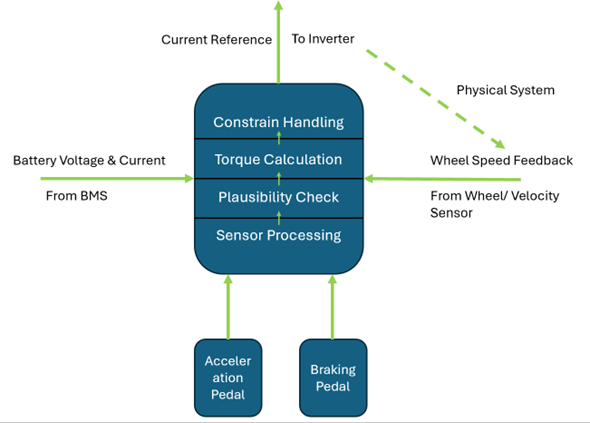
\includegraphics[width=0.5\linewidth]{Block_Diagram_for_Control_System.png}
        \caption{Block Diagram for Control System}
        \label{fig:placeholder}
\end{figure}


The torque request is converted into a current reference signal and sent to the inverter, which regulates motor current to achieve the desired torque output. Feedback mechanisms are incorporated to maintain system stability and traction performance.

\subsubsection{Signal Processing}

The controller processes inputs from multiple sensors, including accelerator and brake pedal signals, wheel speed, and battery measurements.

Raw sensor signals are filtered to reduce noise and ensure stable inputs for control calculations. These processed signals are then used for state estimation and control logic implementation.

\subsubsection{Plausibility and Safety Handling}

Plausibility checks are applied to ensure the validity of critical input signals, particularly the accelerator pedal position sensors. The consistency between multiple pedal signals is monitored to detect implausible conditions in accordance with safety requirements.

If an inconsistency is detected, the torque request is immediately set to zero to ensure safe operation.

In addition, a brake override strategy is implemented, where motor torque is reduced to zero when braking is detected.

\subsubsection{Torque Control Strategy}

The controller calculates the required motor torque based on driver input using a feedforward approach.

The torque demand is converted into a current reference using the motor torque constant. To ensure smooth operation, torque commands are subject to rate limiting to avoid abrupt changes in output.

\subsubsection{Constraint and Feedback Handling}

Feedback from motor and wheel speed is used to monitor system behaviour and estimate slip conditions. When excessive slip is detected, the torque request is reduced to maintain traction.

In addition, system constraints are enforced using battery voltage and current measurements. Power and current limits are applied to ensure operation within the defined electrical constraints.

\subsubsection{Controller Selection}

The controller hardware is selected to support the proposed control strategy while ensuring reliable system operation.

Several platforms were evaluated, including STM32, Arduino Uno, TI C2000, NXP S32K, and Speedgoat/dSPACE systems. After applying basic voltage and communication constraints, a merit matrix is used to compare the feasible options, as shown in Table~\ref{tab:controller_selection}.

\begin{table}[H]
\centering
\caption{Merit Matrix for Controller Selection}
\label{tab:controller_selection}
\begin{tabular}{lcccc}
\toprule
Criteria & STM32 & Arduino Uno & TI C2000 & NXP S32K \\
\midrule
Supply Voltage & Pass & Pass & Pass & Pass \\
Weight & 3 & 1 & 2 & 2 \\
Cost & 3 & 1 & 2 & 2 \\
Processing Time & 1 & 2 & 2 & 1 \\
Latency & 1 & 2 & 2 & 1 \\
CAN Capability & Pass & Fail & Pass & Pass \\
Reliability & 1 & 1 & 1 & 1 \\
\midrule
Overall Score & 15 & 13 & 12 & 12 \\
\bottomrule
\end{tabular}
\end{table}

The results indicate that the STM32 achieves the highest overall score due to its balanced performance in cost, weight, processing capability, communication support, and reliability.

\subsubsection{Final Decision}

Based on the evaluation, the STM32 platform is selected as the controller for the powertrain system.

\subsection{Shutdown Circuit (SDC) Design}

\subsubsection{Overview of Shutdown Circuit}

The shutdown circuit (SDC) is a critical safety system designed to ensure immediate disconnection of the tractive system under fault conditions. It provides fail-safe protection by interrupting the power supply when unsafe conditions are detected.

This ensures that critical safety functions remain reliable even in the event of controller failure.

\subsubsection{Shutdown Circuit Architecture}

The shutdown circuit is designed based on Formula Student UK (FSUK) safety requirements, which mandate a non-programmable, hardware-based system to ensure reliable and fail-safe operation.

The SDC is implemented as a series-connected circuit of safety devices, including monitoring systems and interlock components. All elements must remain in a closed state for normal operation, and any triggered fault will open the circuit and deactivate the tractive system.

\begin{figure}
    \centering
    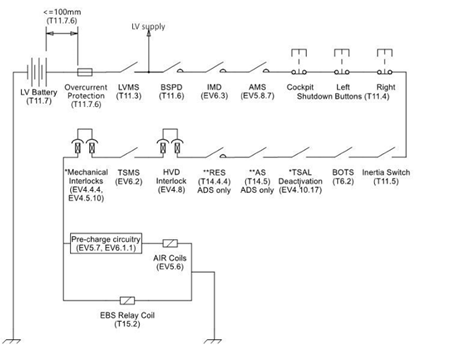
\includegraphics[width=0.5\linewidth]{Shutdown_Circuit_Design.png}
    \caption{ Shutdown Circuit Design}
    \label{fig:placeholder}
\end{figure}

This series configuration ensures that a fault in any individual component will open the entire circuit, resulting in immediate shutdown.

In addition, the circuit is designed such that any loss of power or disconnection will also result in the shutdown circuit opening, ensuring inherently fail-safe behaviour.

\subsubsection{Key Components and Operation}

The shutdown circuit consists of a series of safety-critical components, including monitoring devices and manual shutdown interfaces.

Key elements include the Accumulator Management System (AMS), Insulation Monitoring Device (IMD), Brake System Plausibility Device (BSPD), and shutdown buttons.

Among these, the Accumulator Isolation Relays (AIRs) act as the final switching elements of the shutdown circuit. When the SDC is closed, the AIR coils are energised, allowing the high-voltage system to remain connected.

When any fault condition is detected and the SDC is opened, the AIR coils are de-energised, immediately disconnecting the tractive system.

This ensures that all fault conditions, regardless of their origin, result in a direct and reliable shutdown of the high-voltage system.

\subsection{Drivetrain Design}

\subsubsection{Design Overview}

The drivetrain system is responsible for transmitting torque from the motor to the driven wheels. A chain drive configuration is selected due to its simplicity, low mass, and suitability for short-duration acceleration applications, where efficiency and lightweight design are prioritised.

A typical chain-drive drivetrain consists of a driving and driven sprocket connected by a chain. For the selected YASA P400R motor, which does not include an integrated output shaft, a custom shaft is designed to connect the motor to the drivetrain.

The transmission ratio is determined from simulation, with a final drive ratio of 3:1 selected to balance torque and speed for the acceleration event. Lightweight materials are used to minimise system mass while maintaining sufficient strength.

\subsubsection{Material Selection}

Material selection is performed using a strength-to-weight approach. An Ashby plot of material strength versus density is used to compare candidate materials.

Materials with high strength-to-weight ratios are preferred to minimise mass while maintaining structural integrity.

Due to different loading conditions, different materials are selected for specific components. The output shaft, which is subjected to higher torsional loads, is manufactured using glass fibre reinforced polymer (GFRP) to provide sufficient strength while maintaining low weight.

For the chain and sprocket components, where the loading is comparatively lower, nylon~6 is selected due to its lightweight properties and adequate mechanical performance.

In addition, practical considerations such as cost, reliability, and manufacturability are taken into account to ensure feasibility.

\subsection{Differential Design}

\subsubsection{Design Rationale}

For a straight-line acceleration application, a differential is not strictly required, as both driven wheels can be powered equally.

However, system-level considerations show that incorporating a differential enables a centralised braking configuration. Replacing two wheel-mounted braking systems with a single centralised braking system reduces the overall system mass, despite the addition of the differential.

\subsubsection{Configuration Comparison}

\begin{table}[H]
\centering
\caption{Comparison of Drivetrain Configurations}
\label{tab:drivetrain_comparison}
\begin{tabular}{lcccc}
\toprule
Configuration & Component & Quantity & Weight per Unit (kg) & Total Weight (kg) \\
\midrule
\multirow{3}{*}{No Differential} 
& Braking System & 2 & 3.2 & 6.4 \\
& Differential & 0 & -- & 0 \\
& Total & & & 6.4 \\
\midrule
\multirow{3}{*}{With Differential} 
& Braking System & 1 & 3.2 & 3.2 \\
& Differential & 1 & 2.5 & 2.5 \\
& Total & & & 5.7 \\
\bottomrule
\end{tabular}
\end{table}

The results indicate that the configuration with a differential achieves a lower total system mass.

\subsubsection{Differential Selection}

The differential is selected based on minimising weight and cost while ensuring sufficient torque capacity.

A comparison of candidate options shows that the Drexler FSAE LSD achieves the highest overall score due to its low mass and adequate torque capability. Therefore, it is selected as the most suitable differential for the drivetrain system.

\subsection{Summary}

The powertrain system is designed to maximise acceleration performance under the constraints of the Formula Student competition.

A centralised single-motor architecture is selected to reduce system complexity and mass. The YASA P400R motor is chosen based on its superior torque performance and compatibility with the electrical system.

The inverter selection prioritises voltage range to accommodate the variable output of the supercapacitor system, resulting in the selection of the BAMOCAR PG-D3-700/400.

A structured control system is developed to ensure stable operation, incorporating signal processing, plausibility checks, and constraint handling. Safety is ensured through a shutdown circuit designed in accordance with FSUK requirements.

In addition, system-level optimisation is applied to the mechanical design. A lightweight drivetrain is implemented with a custom output shaft and material selection based on strength-to-weight considerations.

The inclusion of a differential enables a centralised braking configuration, reducing overall system mass.

Overall, the design demonstrates an integrated approach that balances performance, safety, and practicality, resulting in an efficient and competitive powertrain system.

\subsection*{Note}

This section is intentionally left blank to accommodate references and any potential updates or modifications that may be required during subsequent stages of the project.

\end{document}